\documentclass[a4paper]{article}
\usepackage[bottom=2cm]{geometry}
\usepackage{graphicx} 
\usepackage{amsmath}
\usepackage[utf8]{inputenc}
\usepackage{booktabs}
\usepackage{siunitx}
\usepackage{caption}

\title{Relatório A2}
\author{Alice Rabello Oliveira}
\date{Junho 2025}

\begin{document}

\maketitle

\section{Introdução}

\section*{Item 2.1 — Modelo de Geração: Erdős–Rényi}

\subsection*{Metodologia}

\paragraph{Rede 1}
\begin{itemize}
    \item \textbf{Número de nós:} 25
    \item \textbf{Probabilidade de conexão:} \( p = 0{,}2 \)
    \item \textbf{Implementação:} manual em Python.
\end{itemize}

\paragraph{Rede 2}
\begin{itemize}
    \item \textbf{Número de nós:} 25
    \item \textbf{Probabilidade de conexão:} \( p = 0{,}6  \)
    \item \textbf{Implementação:} manual em Python.
\end{itemize}

\paragraph{Rede 3}
\begin{itemize}
    \item \textbf{Número de nós:} 25
    \item \textbf{Probabilidade de conexão:} \( p =  0{,} 8 \)
    \item \textbf{Implementação:} manual em Python.
\end{itemize}


\subsection*{Visualização das Redes}

\begin{center}
    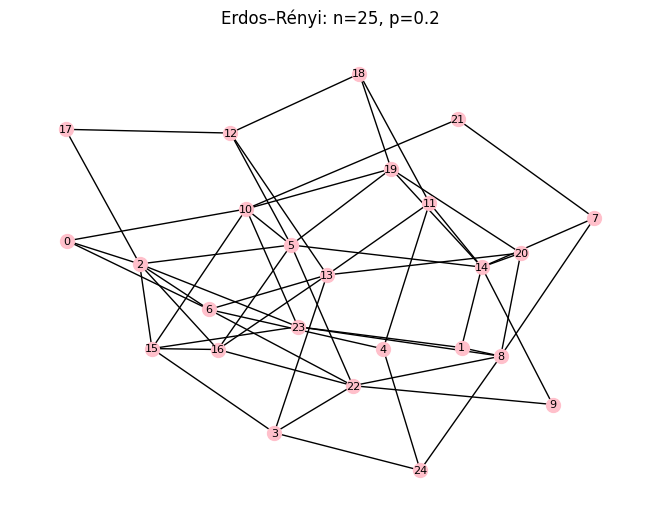
\includegraphics[width=0.6\textwidth]{rede_erdos_t3.png}
\end{center}

\begin{center}
    \includegraphics[width=0.6\textwidth]{Screenshot from 2025-06-12 16-28-45.png}
\end{center}

\begin{center}
    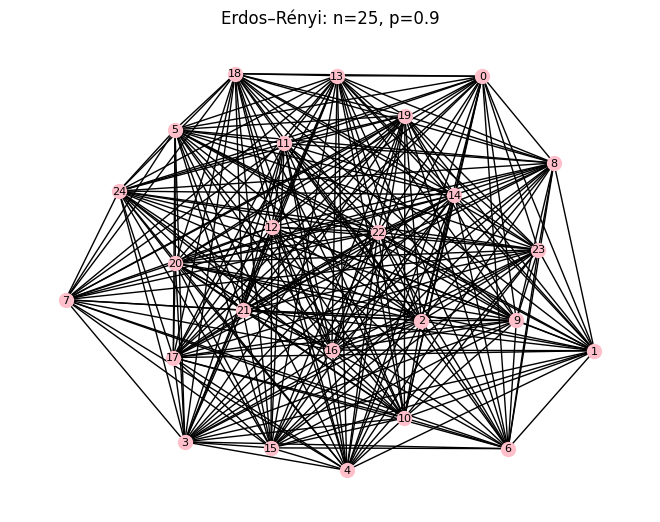
\includegraphics[width=0.6\textwidth]{rede_erdos_t2.png}
\end{center}

Decidi manter um valor razoável da quantidade de nós e observar o comportamento da rede ao alterar o valor de p. É possível observar que, como a formação de uma aresta entre dois nós está sujeita a uma probabilidade p, ao aumentar esse fator, temos que a quantidade de ligações do grafo aumenta em relação ao p escolhido.

\subsection*{Distribuição de Graus}

\begin{center}
    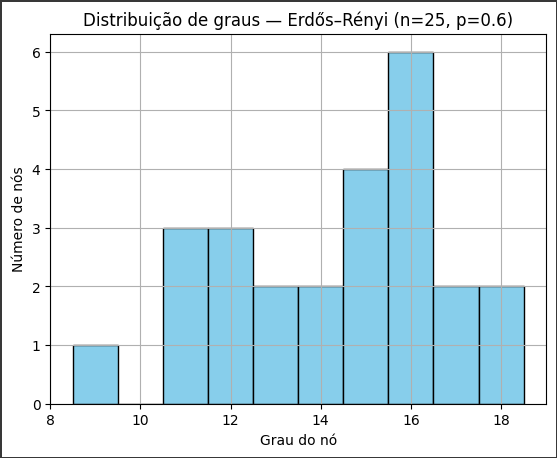
\includegraphics[width=0.5\textwidth]{hist_erdos_t1.png}
\end{center}

\begin{center}
    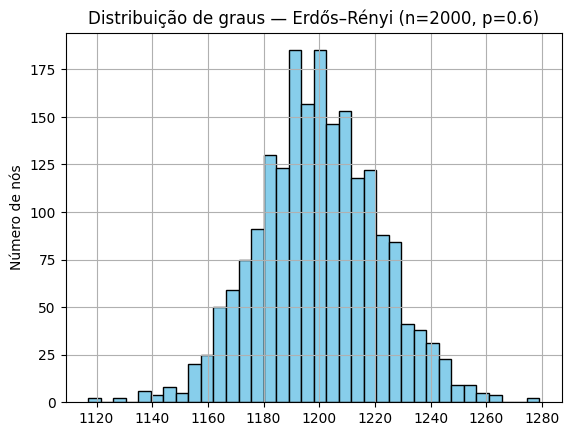
\includegraphics[width=0.5\textwidth]{hist_erdos_t2.png}
\end{center}

\begin{center}
    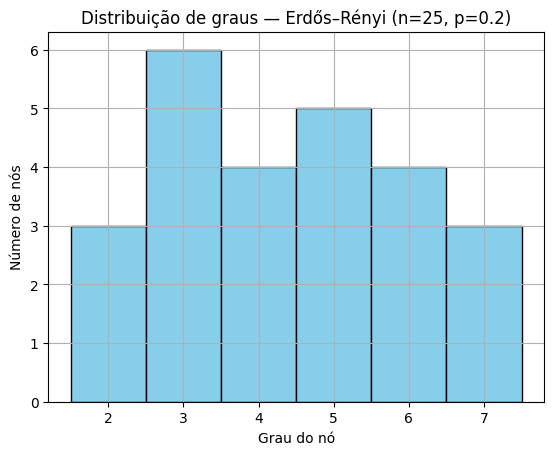
\includegraphics[width=0.5\textwidth]{hist_erdos_t3.png}
\end{center}

Decidi alterar a quantidade de nós com o propósito de ver como a rede se comporta em larga escala. É possível ver que ela segue uma distribuição normal, mesmo que em alguns nós tenham um grau maior; não se configuram como hubs. Temos que os graus estão concentrados na média, de uma forma homogênea. Não existem nós com grau zero e a rede é descentralizada. Essas características são bem comuns na rede que foi analisada, já que a mesma é uma rede aleatória.

\subsection*{Métricas da Rede}

As métricas são das redes em que fiz a visualização, não dos histogramas.
\paragraph{Rede 1}
\begin{itemize}
    \item \textbf{Número de componentes conexas:} 1
    \item \textbf{Diâmetro:} 3
    \item \textbf{Grau médio:} 5.60
    \item \textbf{Coeficiente de clustering médio:} 0.25
    \item \textbf{Densidade:} 0.23
    \item \textbf{Desvio padrão dos graus:} 1.70
    \item \textbf{Caminho médio:} 1.98
    \item \textbf{Quantidade de possíveis hubs:} 1
    \item \textbf{Nó com maior grau:} 4 (grau 9)
\end{itemize}

Como o desvio padrão é baixo, temos que boa parte dos nós tem de 5 a 6 contatos (grau médio de 5.6). O clustering é baixo (0.25), tendo um nó com um grau mais elevado (grau 9). É uma rede conectada, com um nó se destacando. Após melhor análise, vi que o possível hub não é um hub de verdade, devido à origem do modelo analisado.

\paragraph{Rede 2}
\begin{itemize}
    \item \textbf{Número de componentes conexas:} 1
    \item \textbf{Diâmetro:} 2
    \item \textbf{Grau médio:} 13.04
    \item \textbf{Coeficiente de clustering médio:} 0.53
    \item \textbf{Densidade:} 0.54
    \item \textbf{Desvio padrão dos graus:} 2.07
    \item \textbf{Caminho médio:} 1.46
    \item \textbf{Quantidade de possíveis hubs:} nenhum
    \item \textbf{Nó com maior grau:} 23 (grau 17)
\end{itemize}

Temos que é uma rede bem conectada novamente, com qualquer nó a, no máximo, dois saltos de distância de qualquer outro (diâmetro 2). Densa (densidade de 0.54, grau médio de 13.04), com mais da metade das possíveis conexões existentes. Tem um clustering moderado (0.53), o que sugere que os grupos tendem a ser bem interconectados. Desvio padrão baixo (2.07) e sem hubs definidos (nenhum nó com grau significativamente maior que a média) o que nos mostra uma rede homogênea, onde a maioria dos nós possui um número parecido de conexões. 

\paragraph{Rede 3}
\begin{itemize}
    \item \textbf{Número de componentes conexas:} 1
    \item \textbf{Diâmetro:} 2
    \item \textbf{Grau médio:} 19.28
    \item \textbf{Coeficiente de clustering médio:} 0.80
    \item \textbf{Densidade:} 0.80
    \item \textbf{Desvio padrão dos graus:} 1.87
    \item \textbf{Caminho médio:} 1.20
    \item \textbf{Quantidade de possíveis hubs:} nenhum
    \item \textbf{Nó com maior grau:} 0 (grau 23)
\end{itemize}

Temos novamente uma rede totalmente conectada, onde qualquer nó está a no máximo dois saltos de distância de qualquer outro (diâmetro 2). É uma rede bem densa (densidade 0.80, grau médio 19.28), com a grande maioria das possíveis conexões existentes. A rede tem um alto coeficiente de clustering (0.80), o que nos mostra que os grupos internos são fortemente interconectados. O baixo desvio padrão (1.87) e a ausência de hubs definidos (o nó mais conectado tem grau 23, próximo à média) revelam uma rede bastante homogênea, onde praticamente todos os nós possuem número similar de conexões.


\vspace{0.5cm}
\subsection{Código Python para Modelo de Erdos-Rényi}

\begin{verbatim}
import random
import matplotlib.pyplot as plt
import networkx as nx
import numpy as np

def erdos_renyi(n, p):
    # grafo vazio
    G = nx.Graph()
    G.add_nodes_from(range(n))  # nós de 0 até n-1

    # percorre todos os pares (i, j) com i < j
    for i in range(n):
        for j in range(i+1, n):
            if random.random() < p:
                G.add_edge(i, j)

    # desenha o grafo
    nx.draw(
        G,
        with_labels=True,
        node_color='pink',
        edge_color='black',
        node_size=100,
        font_size=8
    )
    plt.title(f"Erdős–Rényi: n={n}, p={p}")
    plt.show()

    graus = [grau for _, grau in G.degree()]
    plt.hist(graus, 
         bins='auto',
         color='skyblue', 
         edgecolor='black')
    plt.title(f"Distribuição de graus — Erdős–Rényi (n={n}, p={p})")
    plt.ylabel("Número de nós")
    plt.grid(True)
    plt.show()

    # metricas
    print("Número de componentes conexas:", nx.number_connected_components(G))
    print(f"Grau médio: {sum(graus) / len(graus):.2f}")
    print(f"Coeficiente de clustering médio: {nx.average_clustering(G):.2f}")
    print(f"Densidade: {nx.density(G):.2f}")
    desvio = np.std([g for n, g in G.degree()])
    print(f"Desvio padrão dos graus: {desvio:.2f}")
    # caminho médio e diâmetro (tratando desconexão)
    if nx.is_connected(G):
        print(f"Caminho médio: {nx.average_shortest_path_length(G):.2f}")
        print(f"Diâmetro: {nx.diameter(G)}")
    else:
        componentes = list(nx.connected_components(G))
        maior_componente = max(componentes, key=len)
        subgrafo = G.subgraph(maior_componente)
        print("Grafo desconexo — analisando maior componente:")
        print(f"Caminho médio: {nx.average_shortest_path_length(subgrafo):.2f}")
        print(f"Diâmetro: {nx.diameter(subgrafo)}")
    # hubs (definido como grau > média + 2 desvios padrão)
    graus_lista = [g for n, g in G.degree()]
    media_grau = np.mean(graus_lista)
    desvio_grau = np.std(graus_lista)
    limite_hub = media_grau + 2 * desvio_grau
    hubs = [n for n, g in G.degree() if g >= limite_hub]
    print(f"Hubs (grau >= {limite_hub:.2f}):", hubs)
    # nó com maior grau
    maior_no = max(G.degree, key=lambda x: x[1])
    print(f"Nó com maior grau: {maior_no[0]} (grau {maior_no[1]})")
\end{verbatim}

\vspace{0.5cm}

\subsection*{Conclusão}

Embora todas as redes tem a propriedade de mundo pequeno, suas estruturas internas variam significativamente. Redes com maior densidade (como a 3 e a 4) tendem a ter caminhos médios menores, enquanto a presença ou ausência de hubs (como na 1 e na 4) vai influenciar diretamente sua organização. O clustering, por sua vez, revela como os nós se agrupam, como por exemplo, redes mais soltas (Rede 2) até comunidades mais interligadas (Rede 3).
Resumind, o modelo testado demonstra como pequenas mudanças nos parâmetros podem gerar redes com dinâmicas distintas: desde estruturas democráticas e equilibradas (Redes 2 e 3) até redes com hubs bem definidos (Redes 1 e 4).

\newpage

\section*{Item 2.2 — Modelo de Geração: Watts–Strogatz}
\subsection*{Metodologia}
\subsubsection{Rede 1}
\begin{itemize}
\item \textbf{Número de nós:} 50
\item \textbf{Grau médio inicial:} k=4
\item \textbf{Probabilidade de rewiring:} p=0
\item \textbf{Implementação:} manual em Python.
\end{itemize}

\subsubsection{Rede 2}
\begin{itemize}
\item \textbf{Número de nós:} 50
\item \textbf{Grau médio inicial:} k=4
\item \textbf{Probabilidade de rewiring:} p=0,1
\item \textbf{Implementação:} manual em Python.
\end{itemize}

\subsubsection{Rede 3}
\begin{itemize}
\item \textbf{Número de nós:} 50
\item \textbf{Grau médio inicial:} k=4
\item \textbf{Probabilidade de rewiring:} p=0,4
\item \textbf{Implementação:} manual em Python.
\end{itemize}

\subsubsection{Rede 4}
\begin{itemize}
\item \textbf{Número de nós:} 50
\item \textbf{Grau médio inicial:} k=4
\item \textbf{Probabilidade de rewiring:} p=0,8
\item \textbf{Implementação:} manual em Python.
\end{itemize}

\subsection*{Visualização da Rede}

\begin{center}
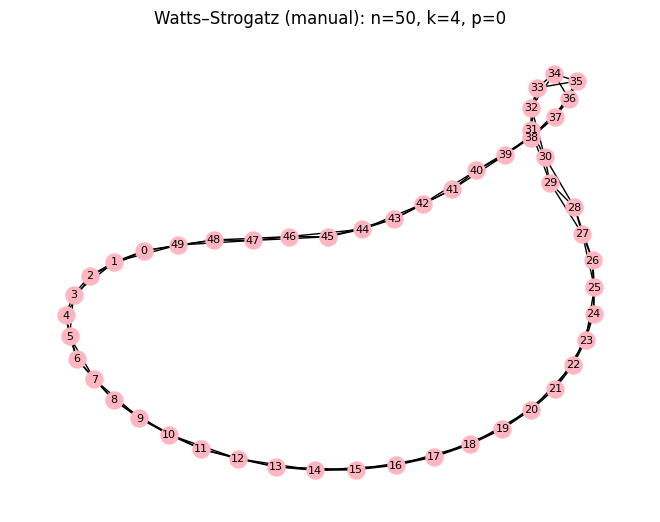
\includegraphics[width=0.6\textwidth]{rede_ws_t1.png}
\end{center}

\begin{center}
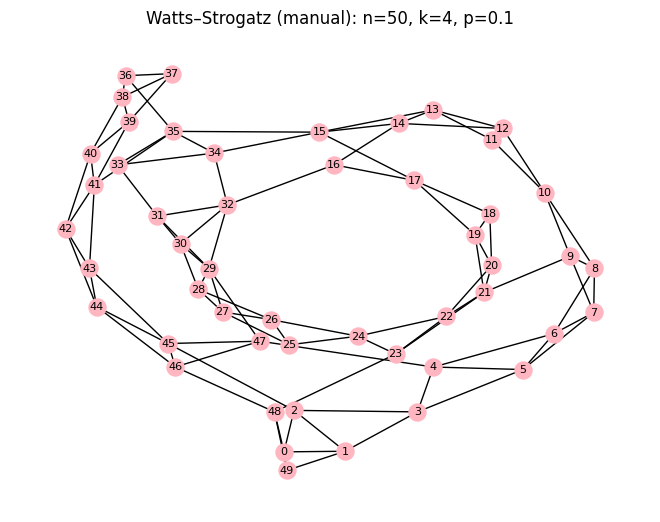
\includegraphics[width=0.6\textwidth]{rede_ws_t2.png}
\end{center}

\begin{center}
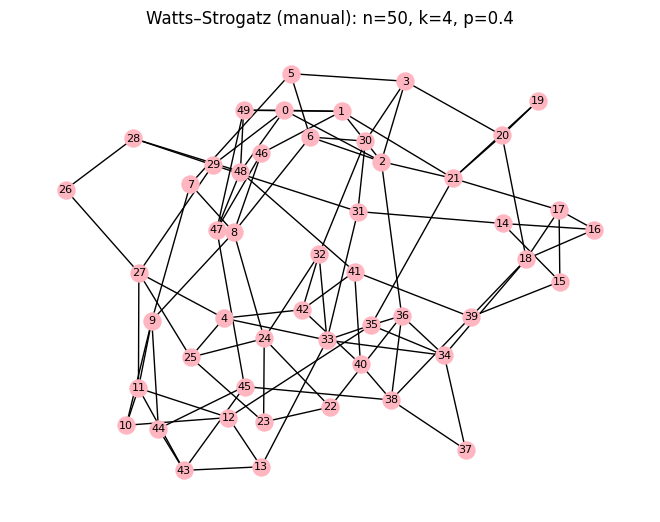
\includegraphics[width=0.6\textwidth]{rede_ws_t3.png}
\end{center}

\begin{center}
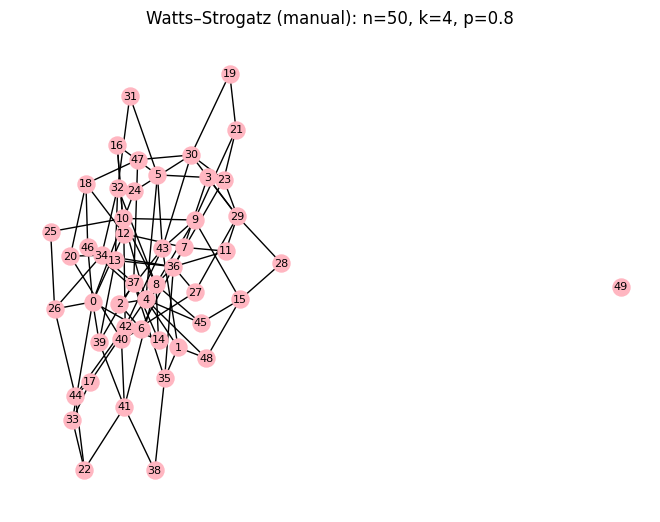
\includegraphics[width=0.6\textwidth]{rede_ws_t4.png}
\end{center}

Nesse modelo, decidi alterar apenas a probabilidade de cada aresta ser “redirecionada” para algum dos outros nós da rede, formando uma rede. A primeira rede apresenta quando esse p é zero, o que mostra apenas uma rede em anel, e nas outras fui variando de probabilidade.

\newpage

\subsection*{Distribuição de Graus}

Na visualização dos histogramas, optei por escolher um k alto e uma quantidade de nós alta, porém com 3 casos diferentes, onde p é baixo, p é médio e p é alto.

\subsubsection{Rede 1}

\begin{figure}[h]
\centering
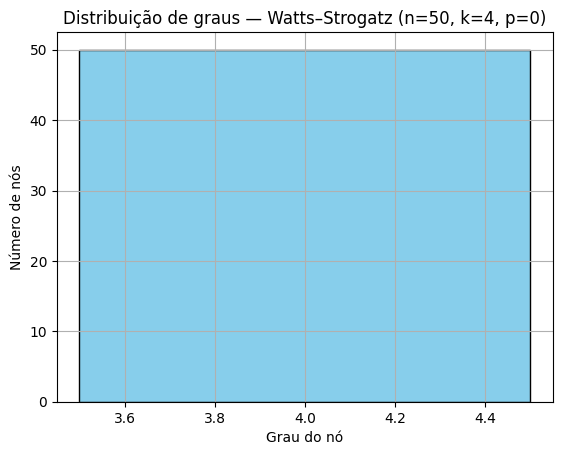
\includegraphics[width=0.6\textwidth]{hist_ws_t1.png}
\end{figure}

\subsubsection{Rede 2}

\begin{figure}[h]
\centering
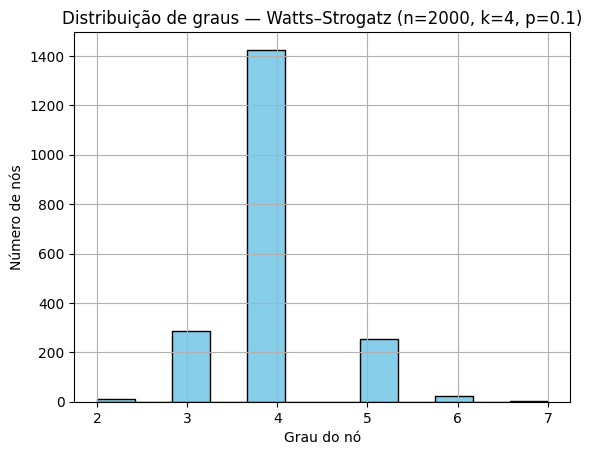
\includegraphics[width=0.6\textwidth]{hist_ws_t2.png}
\end{figure}

\newpage

\subsubsection{Rede 3}

\begin{figure}[h]
\centering
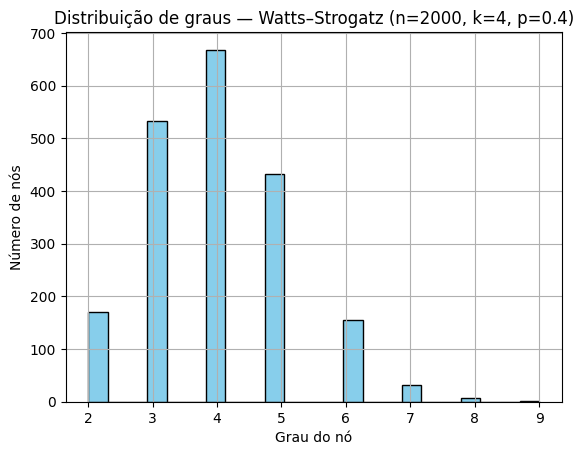
\includegraphics[width=0.6\textwidth]{hist_ws_t3.png}
\end{figure}

Com $p = 0$, todos os nós têm exatamente o mesmo grau. A rede é totalmente regular e o histograma mostra apenas uma barra, o que diz que todos os nós estão conectados da mesma forma.
Podemos perceber como os histogramas quando p tem um valor intermediário, o gráfico assume um formato de distribuição de Poisson.
Quando aumentei para $p = 0{,}6$, os graus começaram a variar. O histograma ainda tem um pico central, mas já mostra mais diversidade. A rede continua organizada, mas com conexões mais aleatórias que diminuem as distâncias, o chamado regime de mundo pequeno.
Com $p = 0{,}9$, a variação aumentou bastante. O histograma ficou bem espalhado, com nós com graus muito diferentes. A rede ficou quase aleatória. Ainda há um centro, mas a estrutura original praticamente desaparece.


\subsection*{Métricas da Rede}

\subsubsection{Rede 1}
As métricas são das redes em que fiz a visualização, não dos histogramas.
\begin{itemize}
    \item \textbf{Número de componentes conexas:} 1
    \item \textbf{Diâmetro:} 13
    \item \textbf{Grau médio:} 4.00
    \item \textbf{Coeficiente de clustering médio:} 0.50
    \item \textbf{Densidade:} 0.08
    \item \textbf{Desvio padrão dos graus:} 0.00
    \item \textbf{Caminho médio:} 6.63
    \item \textbf{Quantidade de possíveis hubs (grau $\geq$ 4.00):} 50
    \item \textbf{Nó com maior grau:} 0 (grau 4)
\end{itemize}

A rede 1 tem uma única componente conexa, diâmetro alto (13) e caminho médio longo (6.63), o que reflete baixa eficiência global. Todos os nós possuem grau 4, sem variação, caracterizando uma rede regular. O clustering médio é relativamente alto (0.50), mas a densidade é baixa (0.08), comum em redes esparsas. Todos os nós são considerados hubs, e o nó com maior grau é o 0, com grau 4.

\subsubsection{Rede 2}
\begin{itemize}
    \item \textbf{Número de componentes conexas:} 1
    \item \textbf{Diâmetro:} 8
    \item \textbf{Grau médio:} 4.00
    \item \textbf{Coeficiente de clustering médio:} 0.38
    \item \textbf{Densidade:} 0.08
    \item \textbf{Desvio padrão dos graus:} 0.49
    \item \textbf{Caminho médio:} 3.85
    \item \textbf{Quantidade de possíveis hubs (grau $\geq$ 4.98):} 6
    \item \textbf{Nó com maior grau:} 1 (grau 5)
\end{itemize}

A rede 2 também é totalmente conectada, mas tem um diâmetro menor (8) e caminho médio mais curto (3.85), o que indica mais eficiência. O grau médio também é 4, com uma leve variação (desvio 0.49). O clustering médio diminui para 0.38 e aparecem 6 hubs (grau ≥ 4.98). O nó mais conectado é o 1, com grau 5.

\subsubsection{Rede 3}
\begin{itemize}
    \item \textbf{Número de componentes conexas:} 1
    \item \textbf{Diâmetro:} 6
    \item \textbf{Grau médio:} 4.00
    \item \textbf{Coeficiente de clustering médio:} 0.17
    \item \textbf{Densidade:} 0.08
    \item \textbf{Desvio padrão dos graus:} 1.33
    \item \textbf{Caminho médio:} 3.01
    \item \textbf{Quantidade de possíveis hubs (grau $\geq$ 6.65):} 3
    \item \textbf{Nó com maior grau:} 46 (grau 8)
\end{itemize}

A rede 3 mantém a conectividade, mas com diâmetro 6 e caminho médio 3.01, o que acaba sendo mais eficiente. O grau médio é 4, mas o desvio sobe para 1.33, o que nos indica forte heterogeneidade. O clustering cai para 0.17 e aparecem 3 hubs (grau ≥ 6.65). O nó mais conectado é o 46, com grau 8.


\subsubsection{Rede 4}

\begin{itemize}
    \item \textbf{Número de componentes conexas:} 1
    \item \textbf{Diâmetro:} 6
    \item \textbf{Grau médio:} 4.00
    \item \textbf{Coeficiente de clustering médio:} 0.08
    \item \textbf{Densidade:} 0.08
    \item \textbf{Desvio padrão dos graus:} 1.39
    \item \textbf{Caminho médio:} 2.90
    \item \textbf{Quantidade de possíveis hubs (grau $\geq$ 6.77):} 3
    \item \textbf{Nó com maior grau:} 31 (grau 8)
\end{itemize}

A rede 4 segue conectada, com diâmetro 6 e caminho médio 2.90, o menor entre todas as redes. O grau médio é 4, com desvio de 1.39, o que mostra a heterogeneidade. O clustering médio é o mais baixo (0.08), quase sem triângulos. Existem 3 hubs (grau ≥ 6.77), e o nó mais conectado é o 31, com grau 8.

\vspace{0.5cm}


\subsection{Código Python para Modelo de Wattz-Strogatz}

\begin{verbatim}
import random
import matplotlib.pyplot as plt
import networkx as nx
import numpy as np

def watts_strogatz(n, k, p):
    if k % 2 != 0:
        raise ValueError("k deve ser par.")

    G = nx.Graph()
    G.add_nodes_from(range(n))

    # conexões do anel regular
    for i in range(n):
        for j in range(1, k//2 + 1):
            neighbor = (i + j) % n
            G.add_edge(i, neighbor)

    # redirecionamento com probabilidade p
    for (i, j) in list(G.edges()):
        if random.random() < p:
            G.remove_edge(i, j)

            possible_nodes = [n for n in range(n) if n != i and not G.has_edge(i, n)]
            if possible_nodes:
                new_target = random.choice(possible_nodes)
                G.add_edge(i, new_target)
            else:
                G.add_edge(i, j)

    # visualização do grafo
    nx.draw(
        G,
        with_labels=True,
        node_size=150,
        font_size=8,
        edge_color='black',
        node_color='lightpink'
    )
    plt.title(f"Watts–Strogatz (manual): n={n}, k={k}, p={p}")
    plt.show()

  # metricas
    print("Número de componentes conexas:", nx.number_connected_components(G))
    graus = [g for _, g in G.degree()]
    print(f"Grau médio: {sum(graus) / len(graus):.2f}")
    print(f"Coeficiente de clustering médio: {nx.average_clustering(G):.2f}")
    print(f"Densidade: {nx.density(G):.2f}")
    desvio = np.std([g for n, g in G.degree()])
    print(f"Desvio padrão dos graus: {desvio:.2f}")
    # caminho médio e diâmetro (tratando desconexão)
    if nx.is_connected(G):
        print(f"Caminho médio: {nx.average_shortest_path_length(G):.2f}")
        print(f"Diâmetro: {nx.diameter(G)}")
    else:
        componentes = list(nx.connected_components(G))
        maior_componente = max(componentes, key=len)
        subgrafo = G.subgraph(maior_componente)
        print("Grafo desconexo — analisando maior componente:")
        print(f"Caminho médio: {nx.average_shortest_path_length(subgrafo):.2f}")
        print(f"Diâmetro: {nx.diameter(subgrafo)}")
    # hubs (definido como grau > média + 2 desvios padrão)
    graus_lista = [g for n, g in G.degree()]
    media_grau = np.mean(graus_lista)
    desvio_grau = np.std(graus_lista)
    limite_hub = media_grau + 2 * desvio_grau
    hubs = [n for n, g in G.degree() if g >= limite_hub]
    print(f"Hubs (grau >= {limite_hub:.2f}):", len(hubs))
    # nó com maior grau
    maior_no = max(G.degree, key=lambda x: x[1])
    print(f"Nó com maior grau: {maior_no[0]} (grau {maior_no[1]})")

    # histograma da distribuição de graus
    plt.hist(graus, 
         bins='auto',
         color='skyblue', 
         edgecolor='black')
    plt.title(f"Distribuição de graus — Watts–Strogatz (n={n}, k={k}, p={p})")
    plt.xlabel("Grau do nó")
    plt.ylabel("Número de nós")
    plt.grid(True)
    plt.show()

    return G

\end{verbatim}

\subsection*{Conclusão}

As redes que foram analisadas mostram a evolução de uma estrutura regular e homogênea (Rede 1), com graus uniformes e alta densidade local, para redes progressivamente mais heterogêneas e eficientes (Redes 2 a 4), onde surgem hubs, o diâmetro e o caminho médio diminuem, e o clustering cai. Isso mostra como a rede vai ficando mais complexa e eficiente, misturando conexões locais fortes com caminhos mais curtos e alguns nós que acabam se tornando mais importantes.

\newpage

\section*{Item 2.3 — Modelo de Geração: Rede com Comunidades}

\subsection*{Metodologia}

\subsubsection{Rede 1}
\begin{itemize}
    \item \textbf{Número de nós:} 100
    \item \textbf{Número de comunidades:} 2
    \item \textbf{Probabilidade de conexão dentro da comunidade:} \(p_{in} = 0{,}3\)
    \item \textbf{Probabilidade de conexão entre comunidades:} \(p_{out} = 0{,}01\)
    \item \textbf{Implementação:} manual, utilizando sorteios para definir as arestas dentro e fora das comunidades.
\end{itemize}

\subsubsection{Rede 2}
\begin{itemize}
    \item \textbf{Número de nós:} 90
    \item \textbf{Número de comunidades:} 3
    \item \textbf{Probabilidade de conexão dentro da comunidade:} \(p_{in} = 0{,}2\)
    \item \textbf{Probabilidade de conexão entre comunidades:} \(p_{out} = 0{,}02\)
    \item \textbf{Implementação:} manual, utilizando sorteios para definir as arestas dentro e fora das comunidades.
\end{itemize}

\subsubsection{Rede 3}
\begin{itemize}
    \item \textbf{Número de nós:} 120
    \item \textbf{Número de comunidades:} 4
    \item \textbf{Probabilidade de conexão dentro da comunidade:} \(p_{in} = 0{,}1\)
    \item \textbf{Probabilidade de conexão entre comunidades:} \(p_{out} = 0{,}05\)
    \item \textbf{Implementação:} manual, utilizando sorteios para definir as arestas dentro e fora das comunidades.
\end{itemize}

\subsubsection{Rede 4}
\begin{itemize}
    \item \textbf{Número de nós:} 100
    \item \textbf{Número de comunidades:} 3
    \item \textbf{Probabilidade de conexão dentro da comunidade:} \(p_{in} = 0{,}4\)
    \item \textbf{Probabilidade de conexão entre comunidades:} \(p_{out} = 0{,}1\)
    \item \textbf{Implementação:} manual, utilizando sorteios para definir as arestas dentro e fora das comunidades.

\newpage

\end{itemize}
\subsection*{Visualização da Rede}

\begin{figure}[h]
\centering
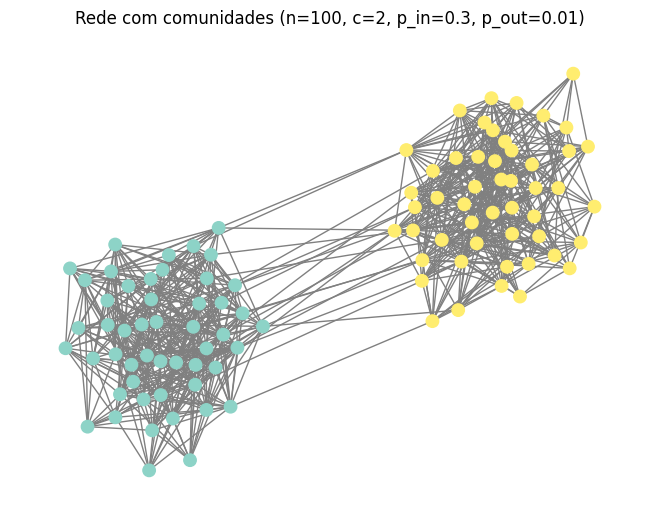
\includegraphics[width=0.6\textwidth]{rede_comunidades_t1.png}
\caption{Rede 1}
\end{figure}

\begin{figure}[h]
\centering
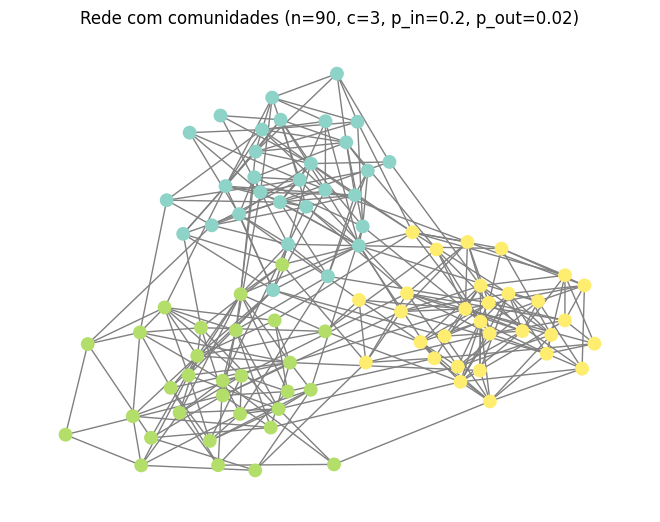
\includegraphics[width=0.6\textwidth]{rede_comunidades_t2.png}
\caption{Rede 2}
\end{figure}

\newpage

\begin{figure}[h]
\centering
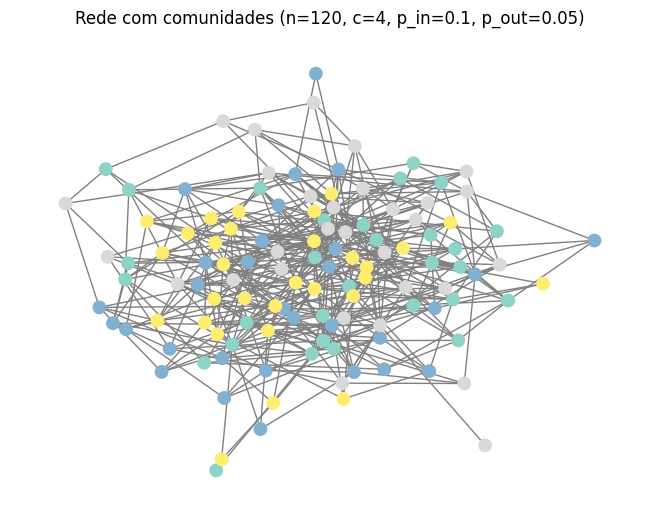
\includegraphics[width=0.6\textwidth]{rede_comunidades_t3.png}
\caption{Rede 3}
\end{figure}

\begin{figure}[h]
\centering
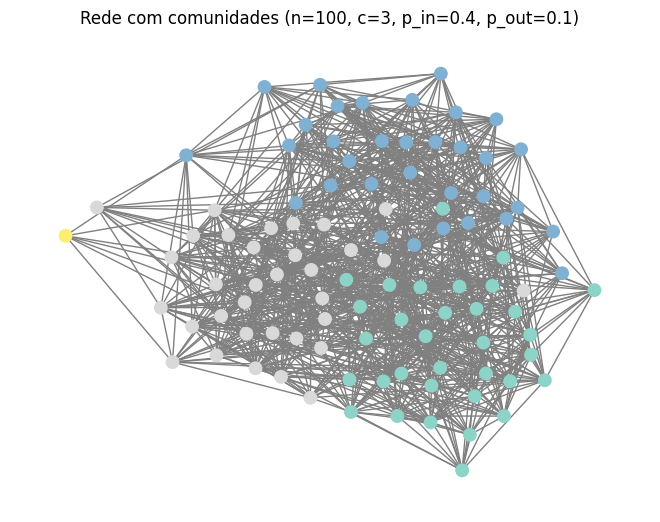
\includegraphics[width=0.6\textwidth]{rede_comunidades_t4.png}
\caption{Rede 4}
\end{figure}


\subsection*{Distribuição de Graus}

Desta vez, os histogramas são das redes visualizadas, então as métricas, histogramas e visualizações são todas relacionadas.

\begin{figure}[h]
\centering
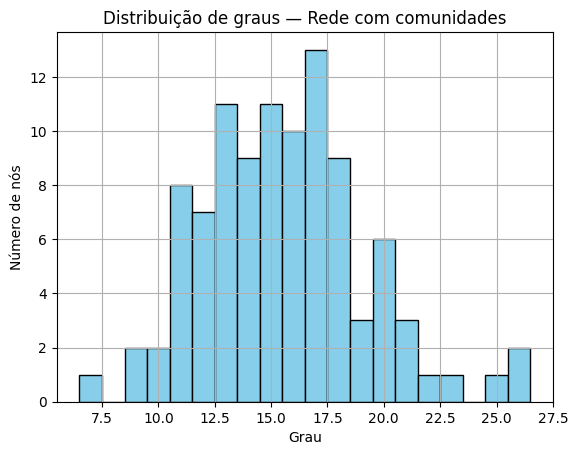
\includegraphics[width=0.6\textwidth]{hist_comunidades_t1.png}
\caption{Distribuição de graus da Rede 1.}
\end{figure}

\begin{figure}[h]
\centering
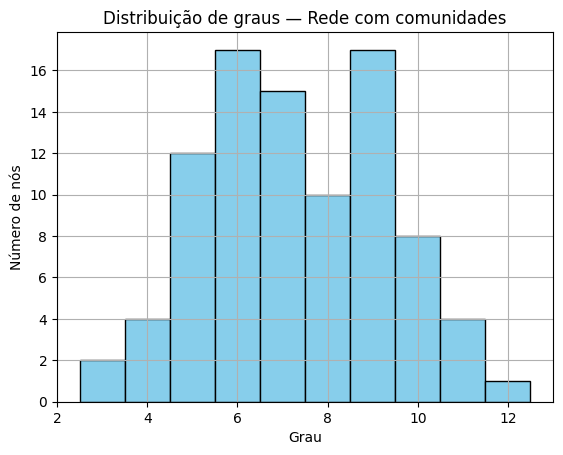
\includegraphics[width=0.6\textwidth]{hist_comunidades_t2.png}
\caption{Distribuição de graus da Rede 2.}
\end{figure}

\newpage

\begin{figure}[h]
\centering
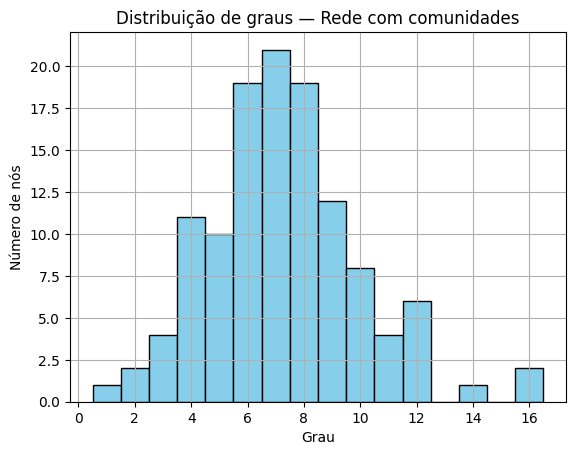
\includegraphics[width=0.6\textwidth]{hist_comunidades_t3.png}
\caption{Distribuição de graus da Rede 3.}
\end{figure}

\begin{figure}[h]
\centering
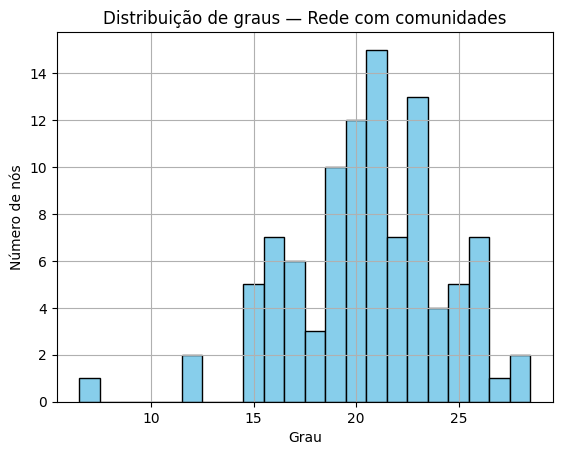
\includegraphics[width=0.6\textwidth]{hist_comunidades_t4.png}
\caption{Distribuição de graus da Rede 4.}
\end{figure}

Foi possível ver como só mudando dois números \(p_{in}\) e \(p_{out}\) a rede muda completamente de comportamento. Os histogramas realmente contam a história da rede, de quando as comunidades são fortes, os graus são mais concentrados e quando a rede é mais “misturada”, o grau se distribui de forma bem mais variada. Isso nos ajuda a entender que só olhar o grafo visualmente às vezes não é suficiente, o histograma ajuda muito a confirmar a estrutura interna.
\newpage

\subsection*{Métricas da Rede}

\subsubsection{Rede 1.}
\begin{itemize}
    \item \textbf{Número de nós:} 100
    \item \textbf{Número de arestas:} 778
    \item \textbf{Número de componentes conexas:} 1
    \item \textbf{Diâmetro:} 4
    \item \textbf{Caminho médio:} 2.27
    \item \textbf{Grau médio:} 15.56
    \item \textbf{Desvio padrão dos graus:} 3.61
    \item \textbf{Coeficiente de clustering médio:} 0.29
    \item \textbf{Densidade:} 0.1572
    \item \textbf{Modularidade (Louvain):} 0.47
\end{itemize}

Nessa rede, os parâmetros com \(p_{in}\) alto e \(p_{out}\) baixo formaram duas comunidades bem definidas. A modularidade é alta (0.47), o clustering também é elevado e o diâmetro é pequeno, o que nos indica boa coesão interna. O histograma mostra graus relativamente concentrados, o que reforça a ideia de blocos fechados.

\subsubsection{Rede 2.}
\begin{itemize}
    \item \textbf{Número de nós:} 90
    \item \textbf{Número de arestas:} 329
    \item \textbf{Número de componentes conexas:} 1
    \item \textbf{Diâmetro:} 5
    \item \textbf{Caminho médio:} 2.64
    \item \textbf{Grau médio:} 7.31
    \item \textbf{Desvio padrão dos graus:} 2.01
    \item \textbf{Coeficiente de clustering médio:} 0.14
    \item \textbf{Densidade:} 0.0821
\end{itemize}

Nessa rede, com três comunidades e menor \(p_{in}\), ela acaba ficando mais diluída. As conexões ainda mostram algum padrão de grupo, mas o clustering é mais baixo (0.14), e a modularidade caiu. O histograma já é mais espalhado, quase uma transição entre estrutura modular e aleatoriedade.

\subsubsection{Rede 3.}
\begin{itemize}
    \item \textbf{Número de nós:} 120
    \item \textbf{Número de arestas:} 437
    \item \textbf{Número de componentes conexas:} 1
    \item \textbf{Diâmetro:} 5
    \item \textbf{Caminho médio:} 2.63
    \item \textbf{Grau médio:} 7.28
    \item \textbf{Desvio padrão dos graus:} 2.68
    \item \textbf{Coeficiente de clustering médio:} 0.07
    \item \textbf{Densidade:} 0.0612
    \item \textbf{Modularidade (Louvain):} 0.32
\end{itemize}

Aqui os valores de \(p_{in}\) e \(p_{out}\) estão próximos, o que faz com que a rede perca praticamente toda a estrutura de comunidades. O clustering é muito baixo (0.07), a modularidade é a menor até agora (0.32), e a distribuição de graus se aproxima da de uma rede aleatória.

\subsubsection{Rede 4.}
\begin{itemize}
    \item \textbf{Número de nós:} 100
    \item \textbf{Número de arestas:} 1029
    \item \textbf{Número de componentes conexas:} 1
    \item \textbf{Diâmetro:} 3
    \item \textbf{Caminho médio:} 1.81
    \item \textbf{Grau médio:} 20.58
    \item \textbf{Desvio padrão dos graus:} 3.68
    \item \textbf{Coeficiente de clustering médio:} 0.24
    \item \textbf{Densidade:} 0.2079
    \item \textbf{Modularidade (Louvain):} 0.30
\end{itemize}

Mesmo com \(p_{in}\) alto, \(p_{out}\) também é relativamente grande, o que gera muitas conexões entre comunidades. A rede é bem conectada (diâmetro 3, caminho médio 1.81), mas a modularidade caiu para 0.30. O grau médio é alto e a densidade também, o que nos mostra que é uma rede densa e bem interligada, com comunidades ainda presentes, mas mais "misturadas".

\newpage

\subsection{Código Python das Redes com Comunidades}

\begin{verbatim}
import networkx as nx
import matplotlib.pyplot as plt
import random
import numpy as np
from collections import Counter

try:
    import community.community_louvain as community_louvain
except:
    community_louvain = None

def rede_comunidades(n=100, c=4, p_in=0.4, p_out=0.02, plot=True):
    G = nx.Graph()
    G.add_nodes_from(range(n))

    # define as comunidades
    tamanho = n // c
    comunidade = {i: i // tamanho for i in range(n)}

    # cria as arestas
    for i in range(n):
        for j in range(i + 1, n):
            if comunidade[i] == comunidade[j]:
                if random.random() < p_in:
                    G.add_edge(i, j)
            else:
                if random.random() < p_out:
                    G.add_edge(i, j)

    # visualização
    if plot:
        cores = [comunidade[n] for n in G.nodes]
        nx.draw(
            G,
            node_color=cores,
            cmap=plt.cm.Set3,
            with_labels=False,
            node_size=80,
            edge_color='gray'
        )
        plt.title(f"Rede com comunidades (n={n}, c={c}, p_in={p_in}, p_out={p_out})")
        plt.show()

    # métricas básicas
    graus = [grau for _, grau in G.degree()]
    print(f"Número de nós: {G.number_of_nodes()}")
    print(f"Número de arestas: {G.number_of_edges()}")
    print(f"Número de componentes conexas: {nx.number_connected_components(G)}")
    
    if nx.is_connected(G):
        print(f"Diâmetro: {nx.diameter(G)}")
        print(f"Caminho médio: {nx.average_shortest_path_length(G):.2f}")
    else:
        maior_componente = max(nx.connected_components(G), key=len)
        Gc = G.subgraph(maior_componente)
        print(f"Caminho médio (maior componente): {nx.average_shortest_path_length(Gc):.2f}")
        print(f"Diâmetro (maior componente): {nx.diameter(Gc)}")
        print(f"Tamanho do maior componente: {len(maior_componente)}")

    print(f"Grau médio: {np.mean(graus):.2f}")
    print(f"Desvio padrão dos graus: {np.std(graus):.2f}")
    print(f"Coeficiente de clustering médio: {nx.average_clustering(G):.2f}")
    print(f"Densidade: {nx.density(G):.4f}")

    # modularidade com Louvain
    if community_louvain is not None:
        partition = community_louvain.best_partition(G)
        modularidade = community_louvain.modularity(partition, G)
        print(f"Modularidade (Louvain): {modularidade:.2f}")
    else:
        print("Biblioteca 'python-louvain' não instalada – modularidade não calculada.")

    # histograma dos graus
    if plot:
        plt.hist(
            graus,
            bins=range(min(graus), max(graus) + 2),
            align='left',
            color='skyblue',
            edgecolor='black'
        )
        plt.title("Distribuição de graus — Rede com comunidades")
        plt.xlabel("Grau")
        plt.ylabel("Número de nós")
        plt.grid(True)
        plt.show()

    return G, comunidade

\end{verbatim}

\subsection*{Conclusão}

Os testes fwitos mostraram que o modelo de comunidades é fortemente influenciado pela diferença entre as probabilidades de ligação interna ($p_{in}$) e externa ($p_{out}$). Quando $p_{in} \gg p_{out}$, as comunidades ficam bem definidas, com alta modularidade e clustering. À medida que $p_{out}$ se aproxima de $p_{in}$, a rede se torna mais aleatória, perdendo a sua estrutura modular. As métricas e histogramas mostram muito bem essa transição, evidenciando como as pequenas variações feitas nos parâmetros impactam bastante a organização da rede.

\newpage

\section*{Item 2.4 — Modelo de Crescimento: Anexação Uniforme}


\subsection*{Metodologia}

\begin{itemize}
    \item \textbf{Rede inicial}: totalmente conectada com 10 nós.
    \item \textbf{Número de novos nós adicionados}: 5
    \item \textbf{Critério de ligação}:
    \begin{itemize}
        \item Em um teste, cada novo nó estabeleceu \textbf{3 ligações fixas} com nós antigos.
        \item Em outro teste, a quantidade de ligações foi \textbf{sorteada aleatoriamente} entre 1 e 4.
    \end{itemize}
    \item \textbf{Implementação}: manual em \texttt{Python} com uso da biblioteca \texttt{networkx}.
\end{itemize}



\subsection*{Diferença entre \textit{m} fixo e \textit{m} aleatório}

Durante os testes, usei duas formas diferentes de definir quantas conexões cada novo nó faz ao entrar na rede. No caso do \textit{m} fixo, todos os novos nós se ligam a exatamente 3 outros. Isso deixa a rede mais equilibrada, com os graus dos nós ficando bem parecidos entre si.

Já no caso do \textit{m} aleatório, o número de conexões varia de nó para nó, sendo sorteado entre 1 e 4. Isso acaba criando uma estrutura mais variada, onde alguns nós acabam com bem mais ou menos conexões que outros. Isso também faz com que a distribuição de graus fique mais espalhada e com maior desvio padrão.

É interessante fazer essa comparação, já que a lógica de crescimento é a mesma, porém o comportamento delas é diferente.

\vspace{0.5cm}

\subsection*{Visualização da Rede Final}

\begin{center}
    \includegraphics[width=0.9\textwidth]{Screenshot from 2025-06-11 18-28-55.png}
\end{center}

\vspace{0.5cm}

\subsection*{Distribuição de Graus}

\begin{center}
    \includegraphics[width=0.9\textwidth]{Screenshot from 2025-06-11 18-29-20.png}
\end{center}

As distribuições mostram a aleatoriedade do modelo. Observamos que os novos nós tendem a ter grau inferior aos nós iniciais. A distribuição não apresenta \textit{hubs}, como é esperado em um modelo de anexação uniforme.

\subsection*{Métricas da Rede}

\begin{table}[h]
\centering
\begin{tabular}{|l|c|c|}
\hline
\textbf{Métrica} & \textbf{m fixo = 3} & \textbf{m aleatório (0-4)} \\
\hline
Número de nós & 15 & 15 \\
Número de arestas & 60 & 57 \\
Grau médio & 8.0 & 7.6 \\
Clustering médio & 0.7780 & 0.6997 \\
Componentes conexas & 1 & 1 \\
Desvio padrão dos graus & 3.37 & 3.57 \\
Densidade & 0.5714 & 0.5429 \\
Caminho médio & 1.46 & 1.49 \\
Diâmetro & 3 & 3 \\
\hline
\end{tabular}
\caption{Métricas calculadas para as duas redes analisadas}
\label{tab:metricas_rede_pequenas}
\end{table}

As duas redes têm o mesmo número de nós, mas diferem um pouco no número de arestas, mostrando pequenas variações na conectividade. O grau médio representa o número médio de conexões por nó, que é alto em ambas as redes, sugerindo uma rede relativamente densa, o que também é confirmado pela densidade próxima a 0,5. O clustering médio mostra que existe uma tendência forte de os vizinhos estarem conectados entre si, o que indica a presença de grupos locais ou triângulos na rede. A única componente conexa confirma que a rede está totalmente conectada, sem ilhas isoladas. O desvio padrão dos graus revela variação moderada na distribuição dos graus dos nós. E por fim, o caminho médio e o diâmetro indicam que a distância entre os nós é pequena, o que caracteriza as redes pequenas e compactas.

\newpage

\subsection{Código Python do Modelo De Anexação Uniforme}

\begin{verbatim}
import networkx as nx
import matplotlib.pyplot as plt
import random
import numpy as np

def anexacao_uniforme(G, n_novos, m=None, aleatorio=False, min_m=1, max_m=3):
    """
    G com n_novos nós, conectando com anexação uniforme.

    parâmetros:
    - G: grafo inicial (NetworkX)
    - n_novos: número de novos nós a adicionar
    - m: número fixo de ligações por novo nó (ignorado se aleatorio=True)
    - aleatorio: se True, sorteia m entre min_m e max_m (inclusive)
    - min_m, max_m: limites de sorteio de m
    """
    proximo_id = max(G.nodes) + 1  # garante IDs únicos para novos nós

    for _ in range(n_novos):
        G.add_node(proximo_id)

        # define quantas conexões esse nó terá
        if aleatorio:
            m_atual = random.randint(min_m, min(max_m, len(G.nodes) - 1))
        else:
            m_atual = min(m, len(G.nodes) - 1)

        # escolhe aleatoriamente os nós existentes para conectar
        possiveis_alvos = list(G.nodes)
        possiveis_alvos.remove(proximo_id)  # não pode conectar com ele mesmo
        alvos = random.sample(possiveis_alvos, m_atual)

        for alvo in alvos:
            G.add_edge(proximo_id, alvo)

        proximo_id += 1

    return G

G_fixo = nx.complete_graph(10)
G_fixo = anexacao_uniforme(G_fixo, n_novos=5, m=3, aleatorio=False)

G_aleat = nx.complete_graph(10)
G_aleat = anexacao_uniforme(G_aleat, n_novos=5, aleatorio=True, min_m=1, max_m=4)

fig, axs = plt.subplots(2, 2, figsize=(12, 10))

# visualização das redes
nx.draw(G_fixo, with_labels=True, node_color='lightblue', ax=axs[0, 0])
axs[0, 0].set_title("Rede com m fixo = 3")

nx.draw(G_aleat, with_labels=True, node_color='lightgreen', ax=axs[0, 1])
axs[0, 1].set_title("Rede com m aleatório (1 a 4)")

# metricas
def imprimir_metricas(G):
    graus = [grau for _, grau in G.degree()]
    print("Número de nós:", G.number_of_nodes())
    print("Número de arestas:", G.number_of_edges())
    print("Grau médio:", np.mean(graus))
    print("Clustering médio:", nx.average_clustering(G))
    print("Componentes conexas:", nx.number_connected_components(G))
    print("Desvio padrão dos graus:", np.std(graus))
    print("Densidade:", nx.density(G))
    print("Caminho médio:", nx.average_shortest_path_length(G))
    print("Diâmetro:\n", nx.diameter(G))


imprimir_metricas(G_fixo)
imprimir_metricas(G_aleat)


# histogramas dos graus
graus_fixo = [grau for _, grau in G_fixo.degree()]
graus_aleat = [grau for _, grau in G_aleat.degree()]

axs[1, 0].hist(graus_fixo, bins=range(min(graus_fixo), max(graus_fixo)+2), align='left', color='skyblue', edgecolor='black')
axs[1, 0].set_title("Distribuição de graus (m fixo)")
axs[1, 0].set_xlabel("Grau")
axs[1, 0].set_ylabel("Número de nós")

axs[1, 1].hist(graus_aleat, bins=range(min(graus_aleat), max(graus_aleat)+2), align='left', color='lightgreen', edgecolor='black')
axs[1, 1].set_title("Distribuição de graus (m aleatório)")
axs[1, 1].set_xlabel("Grau")
axs[1, 1].set_ylabel("Número de nós")

plt.tight_layout()
plt.show()


\end{verbatim}

\subsection*{Conclusão}
O modelo de anexação uniforme, como o esperado, gerou uma rede sem \textit{hubs} e com distribuição de graus assimétrica. As métricas calculadas (como alto clustering e baixo caminho médio) mostram a influência da rede inicial totalmente conectada. Este comportamento faz um contraste com modelos baseados em anexação preferencial, onde a heterogeneidade de graus é mais destacada.

\newpage

\section*{Item 2.5 — Modelo de Crescimento: Anexação Preferencial}

\subsection*{Metodologia}

\begin{itemize}
    \item \textbf{Rede inicial:} totalmente conectada com 10 nós.
    \item \textbf{Número de novos nós adicionados:} 90
    \item \textbf{Critério de ligação:}
    \begin{itemize}
        \item Em um teste, cada novo nó estabeleceu 3 ligações fixas com nós antigos.
        \item Em outro teste, a quantidade de ligações foi sorteada aleatoriamente entre 1 e 4.
    \end{itemize}
    \item \textbf{Implementação:} desenvolvida manualmente em Python com uso da biblioteca \texttt{networkx} apenas para análise e visualização.
\end{itemize}

\subsection*{Visualização da Rede Final}

\begin{center}
    \includegraphics[width=0.8\textwidth]{Screenshot from 2025-06-11 18-38-08.png}
\end{center}

\vspace{0.5cm}
\subsection*{Distribuição de Graus}

\begin{center}
    \includegraphics[width=0.8\textwidth]{Screenshot from 2025-06-11 18-39-30.png}
\end{center}

A distribuição de graus das redes geradas apresentam \textbf{cauda longa}, com a maioria dos nós tendo poucos vizinhos e poucos nós concentrando um grande número de conexões (\textit{hubs}). Esse comportamento é característico de redes \textit{livre de escala} (distribuição do grau por nó segue uma lei de potência).

\newpage

\subsection*{Diferença entre $m$ fixo e $m$ aleatório}

Nos testes com o modelo de anexação preferencial, usei tanto o $m$ fixo quanto o aleatório. Quando mantive $m = 3$, cada novo nó fazia exatamente 3 conexões. Mesmo assim, a rede formou \textit{hubs} naturalmente, já que os nós mais conectados continuam sendo os mais atrativos para novas ligações.

Quando usei $m$ aleatório, sorteando entre 1 e 4 conexões por novo nó, a rede ficou mais desigual. A distribuição de graus se espalhou mais e o desvio padrão aumentou. Essa variação deixou a rede com uma estrutura ainda mais assimétrica e imprevisível, mesmo mantendo o mesmo tipo de anexação.

Em ambos os casos, a estrutura resultante tende a se organizar com \textbf{nós altamente conectados (hubs)}, o que é uma característica marcante desse tipo de modelo.

\subsection*{Métricas da Rede}

\begin{table}[h]
\centering
\begin{tabular}{|l|c|c|}
\hline
\textbf{Métrica} & \textbf{m fixo = 3} & \textbf{m aleatório (1–4)} \\
\hline
Número de nós & 100 & 100 \\
Número de arestas & 315 & 271 \\
Grau médio & 6.3 & 5.42 \\
Clustering médio & 0.2930 & 0.2231 \\
Componentes conexas & 1 & 1 \\
Desvio padrão dos graus & 6.55 & 6.13 \\
Densidade & 0.0636 & 0.0547 \\
Caminho médio & 2.49 & 2.69 \\
Diâmetro & 5 & 6 \\
\hline
\end{tabular}
\caption{Métricas calculadas para as duas variações da rede}
\label{tab:metricas_rede}
\end{table}

As duas redes possuem mesma quantidade de nós e uma única componente conexa, indicando que todos os nós estão interligados direta ou indiretamente. O número de arestas e o grau médio são relativamente baixos, o que é típico do modelo, que vai gerar redes esparsas. A densidade também é baixa, o que reforça essa característica. O clustering médio é moderado, o que é esperado nesse modelo, já que os novos nós se conectam preferencialmente a nós de alto grau, favorecendo a formação de hubs, mas não necessariamente triângulos. O desvio padrão dos graus é alto, refletindo a distribuição desigual de conexões, uma marca do modelo: poucos nós com grau alto (hubs) e muitos com grau baixo. Por fim, os caminhos médios curtos e os diâmetros pequenos destacam a propriedade de pequeno mundo, comum em redes com estrutura de hubs.

\newpage

\subsection{Código Python do Modelo de Anexação Preferencial}

\begin{verbatim}
import networkx as nx
import matplotlib.pyplot as plt
import random
import numpy as np

def anexacao_preferencial(G, n_novos, m=None, aleatorio=False, min_m=1, max_m=3):
    """
    rede G com anexação preferencial (modelo Barabási-Albert).

    parâmetros:
    - G: grafo inicial (NetworkX)
    - n_novos: número de novos nós a adicionar
    - m: número fixo de ligações por novo nó (ignorado se aleatorio=True)
    - aleatorio: se True, sorteia m entre min_m e max_m (inclusive)
    - min_m, max_m: limites de sorteio de m
    """
    proximo_id = max(G.nodes) + 1

    for _ in range(n_novos):
        G.add_node(proximo_id)

        # define quantas conexões esse nó terá
        if aleatorio:
            m_atual = random.randint(min_m, min(max_m, len(G.nodes) - 1))
        else:
            m_atual = min(m, len(G.nodes) - 1)

        # calcular graus acumulados para anexação preferencial
        graus = np.array([G.degree(n) for n in G.nodes if n != proximo_id])
        nos_existentes = [n for n in G.nodes if n != proximo_id]

        if graus.sum() == 0:
            # todos com probabilidade igual se graus forem todos zero
            alvos = random.sample(nos_existentes, m_atual)
        else:
            probabilidades = graus / graus.sum()
            alvos = np.random.choice(nos_existentes, size=m_atual, replace=False, p=probabilidades)

        for alvo in alvos:
            G.add_edge(proximo_id, alvo)

        proximo_id += 1

    return G

# grafo inicial completamente conectado
G_fixo = nx.complete_graph(10)
G_fixo = anexacao_preferencial(G_fixo, n_novos=90, m=3, aleatorio=False)

G_aleat = nx.complete_graph(10)
G_aleat = anexacao_preferencial(G_aleat, n_novos=90, aleatorio=True, min_m=1, max_m=4)

# metricas
def imprimir_metricas(G):
    graus = [grau for _, grau in G.degree()]
    print("Número de nós:", G.number_of_nodes())
    print("Número de arestas:", G.number_of_edges())
    print("Grau médio:", np.mean(graus))
    print("Clustering médio:", nx.average_clustering(G))
    print("Componentes conexas:", nx.number_connected_components(G))
    print("Desvio padrão dos graus:", np.std(graus))
    print("Densidade:", nx.density(G))
    print("Caminho médio:", nx.average_shortest_path_length(G))
    print("Diâmetro:\n", nx.diameter(G))


imprimir_metricas(G_fixo)
imprimir_metricas(G_aleat)


# visualização
fig, axs = plt.subplots(2, 2, figsize=(12, 10))

nx.draw(G_fixo, with_labels=False, node_color='lightblue', node_size=50, ax=axs[0, 0])
axs[0, 0].set_title("Anexação preferencial (m fixo = 3)")

nx.draw(G_aleat, with_labels=False, node_color='lightgreen', node_size=50, ax=axs[0, 1])
axs[0, 1].set_title("Anexação preferencial (m aleatório 1–4)")

graus_fixo = [grau for _, grau in G_fixo.degree()]
graus_aleat = [grau for _, grau in G_aleat.degree()]

axs[1, 0].hist(graus_fixo, bins=range(min(graus_fixo), max(graus_fixo)+2), align='left', color='skyblue', edgecolor='black')
axs[1, 0].set_title("Distribuição de graus (m fixo)")
axs[1, 0].set_xlabel("Grau")
axs[1, 0].set_ylabel("Número de nós")

axs[1, 1].hist(graus_aleat, bins=range(min(graus_aleat), max(graus_aleat)+2), align='left', color='lightgreen', edgecolor='black')
axs[1, 1].set_title("Distribuição de graus (m aleatório)")
axs[1, 1].set_xlabel("Grau")
axs[1, 1].set_ylabel("Número de nós")

plt.tight_layout()
plt.show()
\end{verbatim}

\subsection*{Conclusão}

O modelo resultou em redes com \textbf{hubs naturais}, onde poucos nós concentram grande parte das conexões. Isso causa um contraste forte com o modelo de anexação uniforme, no qual a distribuição de graus é mais homogênea.
Além disso, o clustering médio tende a ser menor, e o desvio padrão dos graus significativamente maior, o que mostra a \textbf{heterogeneidade estrutural} da rede.

\newpage

\section*{Item 2.6 — Modelo de Crescimento: Modelo de Price}

\subsection*{Metodologia}

\begin{itemize}
    \item \textbf{Rede inicial:} totalmente conectada com 10 nós.
    \item \textbf{Número de novos nós adicionados:} 90.
    \item \textbf{Critério de ligação:}
    \begin{itemize}
        \item Em um teste, cada novo nó estabeleceu 3 ligações fixas com nós antigos (\(m = 3\)).
        \item Em outro teste, o número de ligações foi sorteado aleatoriamente entre 1 e 4.
    \end{itemize}
    \item \textbf{Parâmetro de controle:} 60\% das ligações foram feitas via anexação preferencial, e 40\% de forma uniforme (\(\text{preferência} = 0.6\)).
    \item \textbf{Implementação:} desenvolvida manualmente em Python com uso da biblioteca \texttt{networkx} apenas para análise e visualização. A lógica de crescimento foi programada diretamente.
\end{itemize}

\subsection*{Visualização da Rede Final}

\subsubsection{Redes 1}
\begin{figure}[h]
\begin{center}
    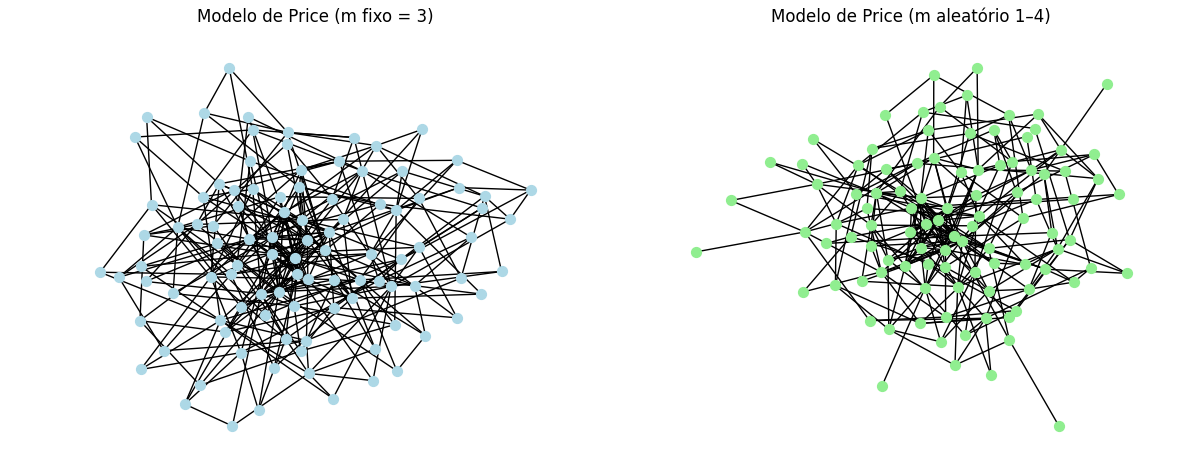
\includegraphics[width=0.8\textwidth]{rede_price_t1.png}
\end{center}
\caption{Redes geradas com o modelo de Price: à esquerda com \(m = 3\), à direita com \(m\) sorteado entre 1 e 4; p = 0.}
\end{figure}

\subsubsection{Redes 2}
\begin{figure}[h]
\begin{center}
    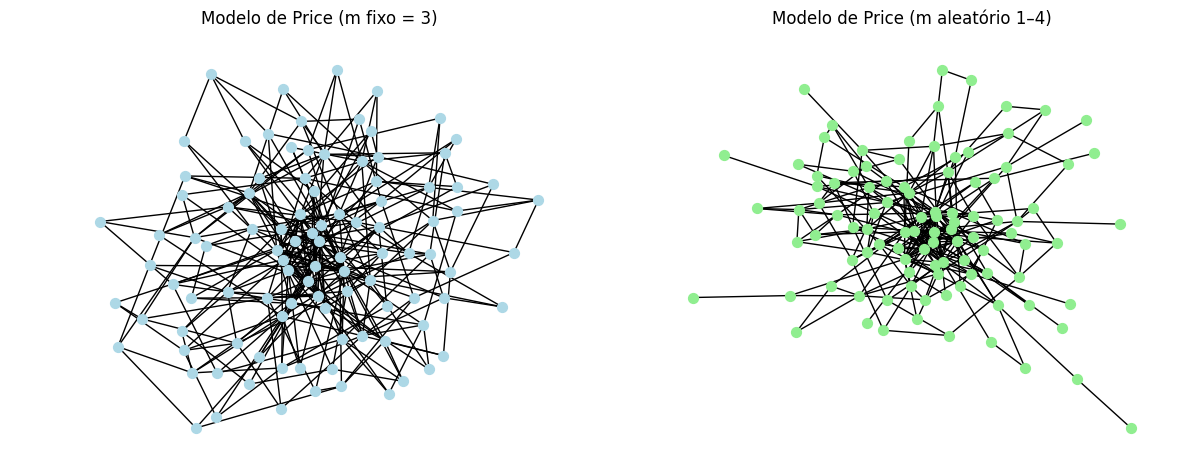
\includegraphics[width=0.8\textwidth]{rede_price_t2.png}
\end{center}
\caption{Redes geradas com o modelo de Price: à esquerda com \(m = 3\), à direita com \(m\) sorteado entre 1 e 4; p = 0,6.}
\end{figure}

\subsubsection{Redes 3}
\begin{figure}[h]
\begin{center}
    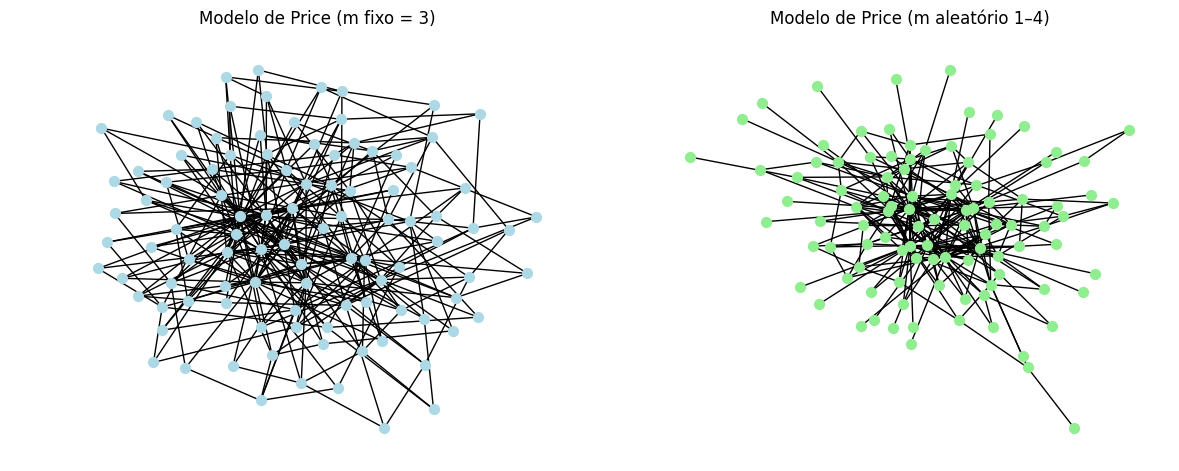
\includegraphics[width=0.8\textwidth]{rede_price_t3.png}
\end{center}
\caption{Redes geradas com o modelo de Price: à esquerda com \(m = 3\), à direita com \(m\) sorteado entre 1 e 4; p = 1.0.}
\end{figure}

\subsection*{Distribuição de Graus}

\subsubsection{Rede 1}

\begin{figure}[h]
\begin{center}
    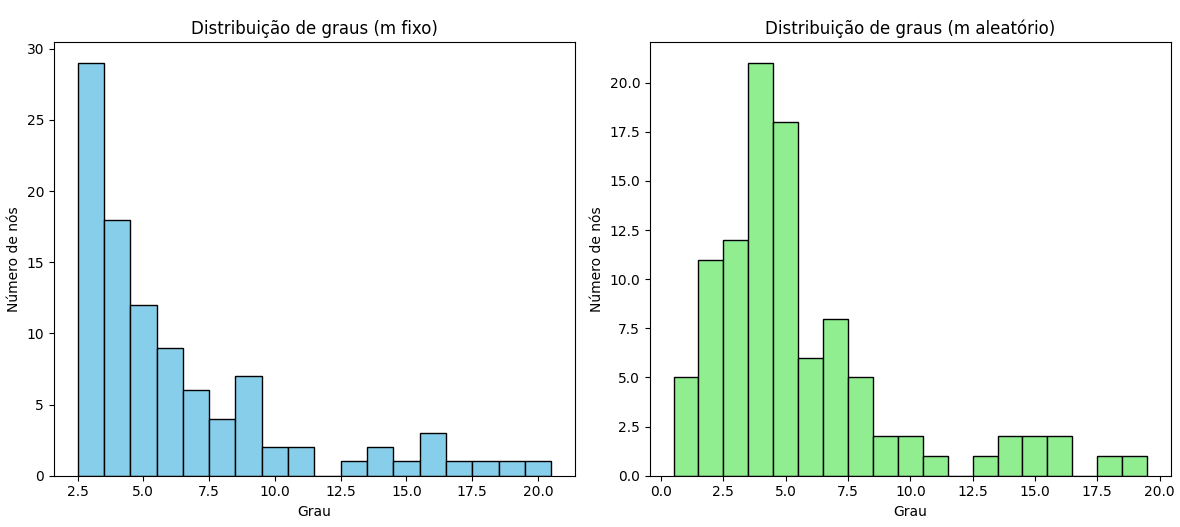
\includegraphics[width=0.8\textwidth]{hist_price_t1.png}
\end{center}
\caption{Distribuição de graus para as redes 1.}
\end{figure}

\newpage

\subsubsection{Rede 2}

\begin{figure}[h]
\begin{center}
    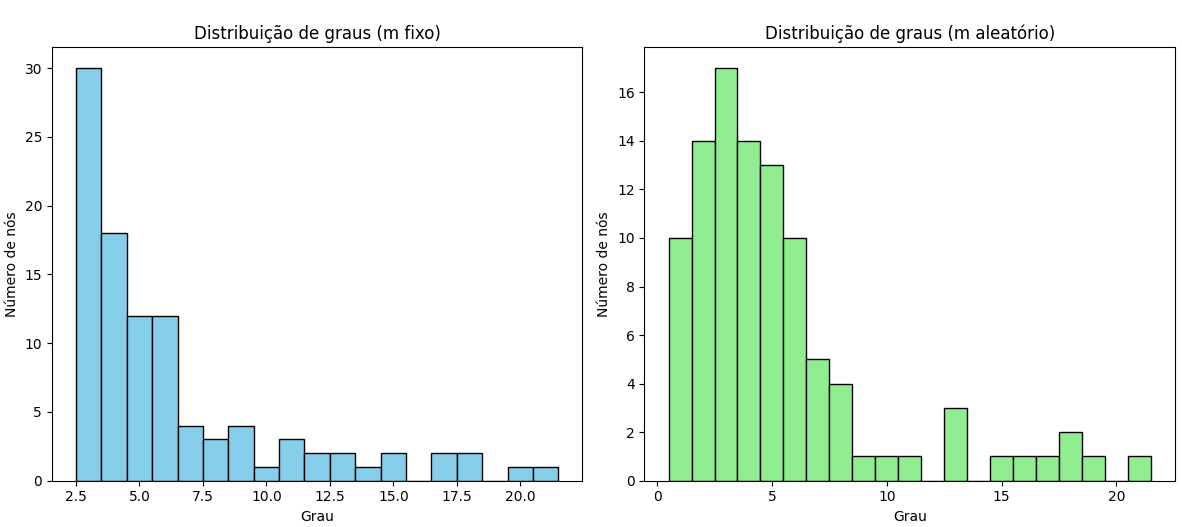
\includegraphics[width=0.8\textwidth]{hist_price_t2.png}
\end{center}
\caption{Distribuição de graus paras redes 2.}
\end{figure}

\subsubsection{Rede 3}

\begin{figure}[h]
\begin{center}
    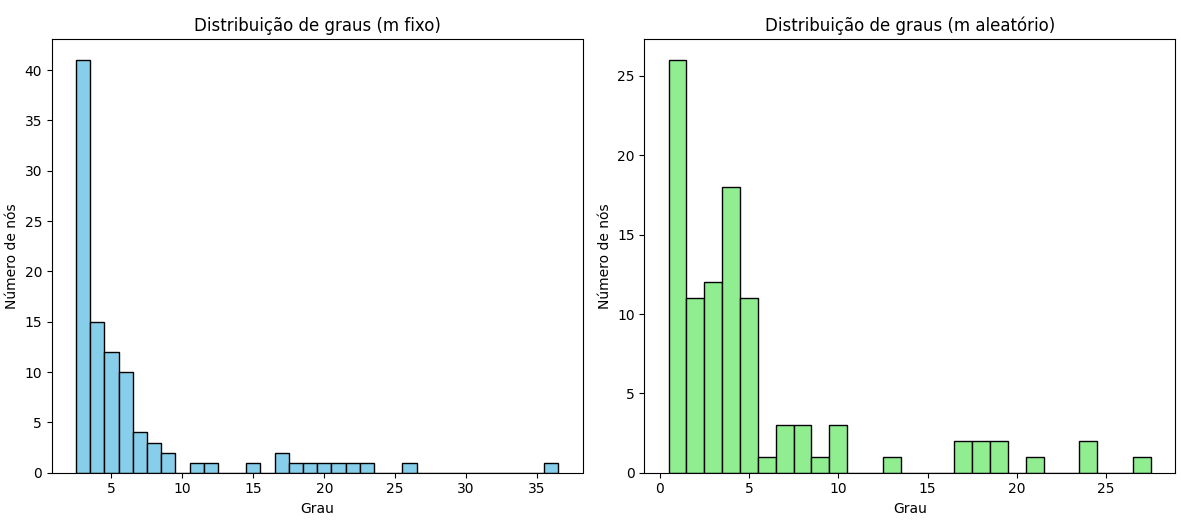
\includegraphics[width=0.8\textwidth]{hist_price_t3.png}
\end{center}
\caption{Distribuição de graus para as redes 3.}
\end{figure}

As distribuições de graus mostram um padrão intermediário entre o modelo de anexação uniforme e o modelo preferencial puro. A presença de alguns hubs é visível, mas com menor intensidade do que no modelo de Barabási–Albert.

\subsection*{Métricas da Rede}

\subsubsection{Redes 1}

\begin{table}[h]
\centering
\begin{tabular}{|l|c|c|}
\hline
\textbf{Métrica} & \textbf{m fixo = 3} & \textbf{m aleatório (1–4)} \\
\hline
Número de nós & 100 & 100 \\
Número de arestas & 315 & 276 \\
Grau médio & 6.30 & 5.52 \\
Clustering médio & 0.11 & 0.11 \\
Componentes conexas & 1 & 1 \\
Desvio padrão dos graus & 3.74 & 4.03 \\
Densidade & 0.0636 & 0.0558 \\
Caminho médio & 2.76 & 3.00 \\
Diâmetro & 5 & 6 \\
\hline
\end{tabular}
\caption{Métricas calculadas para as redes 1 geradas com o modelo de Price.}
\end{table}

As duas redes têm o mesmo número de nós e componentes, mas com m fixo, o grau médio foi um pouco maior e a rede ficou mais compacta (menor caminho médio e diâmetro). Com m aleatório, a variação de graus aumentou, o que deixa a rede mais espalhada. O clustering médio foi igual nos dois casos, o que mostra que a estrutura local se manteve parecida.

\newpage 

\subsubsection{Rede 2}
\begin{table}[h]
\centering
\begin{tabular}{|l|c|c|}
\hline
\textbf{Métrica} & \textbf{m fixo = 3} & \textbf{m aleatório (1–4)} \\
\hline
Número de nós & 100 & 100 \\
Número de arestas & 315 & 265 \\
Grau médio & 6.30 & 5.30 \\
Clustering médio & 0.11 & 0.12 \\
Componentes conexas & 1 & 1 \\
Desvio padrão dos graus & 4.28 & 4.30 \\
Densidade & 0.0636 & 0.0535 \\
Caminho médio & 2.70 & 3.01 \\
Diâmetro & 5 & 6 \\
\hline
\end{tabular}
\caption{Métricas calculadas para as redes 2 geradas com o modelo de Price.}
\end{table}

Com m fixo, a rede ficou um pouco mais densa e compacta, com menor caminho médio. Já com m aleatório, o grau médio caiu, o diâmetro aumentou e a rede ficou um pouco mais espalhada. A variação dos graus foi parecida nos dois casos, mas o clustering médio subiu um pouco mais com m aleatório.

\subsubsection{Rede 3}
\begin{table}[h]
\centering
\begin{tabular}{|l|c|c|}
\hline
\textbf{Métrica} & \textbf{m fixo = 3} & \textbf{m aleatório (1–4)} \\
\hline
Número de nós & 100 & 100 \\
Número de arestas & 315 & 259 \\
Grau médio & 6.30 & 5.18 \\
Clustering médio & 0.23 & 0.15 \\
Componentes conexas & 1 & 1 \\
Desvio padrão dos graus & 5.86 & 5.70 \\
Densidade & 0.0636 & 0.0523 \\
Caminho médio & 2.53 & 2.77 \\
Diâmetro & 4 & 6 \\
\hline
\end{tabular}
\caption{Métricas calculadas para as redes 3 (preferência = 1) geradas com o modelo de Price.}
\end{table}

Com p = 1, a rede ficou bem desigual, o desvio dos graus é alto nos dois casos, mostrando que hubs surgiram com força. A versão com m fixo teve maior clustering e menor diâmetro, o que forma uma estrutura mais conectada. Já a com m aleatório ficou mais dispersa, com menos conexões e maior diâmetro. Foi a rede com maior variação até agora, onde dá pra ver claramente a influência da anexação preferencial.

\subsection{Código Python do Modelo de Price}

\begin{verbatim}
import networkx as nx
import matplotlib.pyplot as plt
import random
import numpy as np

def modelo_price(G, n_novos, m=None, aleatorio=False, min_m=1, max_m=3, preferencia=0.5):
    """
    rede G com o modelo de Price: parte preferencial, parte uniforme.

    parâmetros:
    - G: grafo inicial (NetworkX)
    - n_novos: número de novos nós a adicionar
    - m: número fixo de ligações por novo nó (ignorado se aleatorio=True)
    - aleatorio: se True, sorteia m entre min_m e max_m (inclusive)
    - preferencia: proporção das ligações feitas com anexação preferencial (entre 0 e 1)
    """
    proximo_id = max(G.nodes) + 1

    for _ in range(n_novos):
        G.add_node(proximo_id)

        # define quantas conexões esse nó terá
        if aleatorio:
            m_atual = random.randint(min_m, min(max_m, len(G.nodes) - 1))
        else:
            m_atual = min(m, len(G.nodes) - 1)

        # separa quantidade de conexões preferenciais e uniformes
        m_pref = int(preferencia * m_atual)
        m_uni = m_atual - m_pref

        # nós existentes, sem o novo nó
        nos_existentes = [n for n in G.nodes if n != proximo_id]

        # anexação preferencial
        alvos_pref = []
        if m_pref > 0:
            graus = np.array([G.degree(n) for n in nos_existentes])
            if graus.sum() == 0:
                alvos_pref = random.sample(nos_existentes, m_pref)
            else:
                probs = graus / graus.sum()
                alvos_pref = list(np.random.choice(nos_existentes, size=m_pref, replace=False, p=probs))

        # anexação uniforme
        alvos_restantes = list(set(nos_existentes) - set(alvos_pref))
        alvos_uni = random.sample(alvos_restantes, min(m_uni, len(alvos_restantes)))

        # adiciona as arestas
        for alvo in alvos_pref + alvos_uni:
            G.add_edge(proximo_id, alvo)

        proximo_id += 1

    return G

# redes iniciais
G_fixo = nx.complete_graph(10)
G_aleat = nx.complete_graph(10)

# modelo de Price
G_fixo = modelo_price(G_fixo, n_novos=90, m=3, preferencia=0.6, aleatorio=False)
G_aleat = modelo_price(G_aleat, n_novos=90, aleatorio=True, min_m=1, max_m=4, preferencia=0.6)

# visualização e análise
fig, axs = plt.subplots(2, 2, figsize=(12, 10))

nx.draw(G_fixo, with_labels=False, node_color='lightblue', node_size=50, ax=axs[0, 0])
axs[0, 0].set_title("Modelo de Price (m fixo = 3)")

nx.draw(G_aleat, with_labels=False, node_color='lightgreen', node_size=50, ax=axs[0, 1])
axs[0, 1].set_title("Modelo de Price (m aleatório 1–4)")

graus_fixo = [grau for _, grau in G_fixo.degree()]
graus_aleat = [grau for _, grau in G_aleat.degree()]

axs[1, 0].hist(graus_fixo, bins=range(min(graus_fixo), max(graus_fixo)+2), align='left', color='skyblue', edgecolor='black')
axs[1, 0].set_title("Distribuição de graus (m fixo)")
axs[1, 0].set_xlabel("Grau")
axs[1, 0].set_ylabel("Número de nós")

axs[1, 1].hist(graus_aleat, bins=range(min(graus_aleat), max(graus_aleat)+2), align='left', color='lightgreen', edgecolor='black')
axs[1, 1].set_title("Distribuição de graus (m aleatório)")
axs[1, 1].set_xlabel("Grau")
axs[1, 1].set_ylabel("Número de nós")

plt.tight_layout()
plt.show()

def imprimir_metricas(G):
    graus = [grau for _, grau in G.degree()]
    print("Número de nós:", G.number_of_nodes())
    print("Número de arestas:", G.number_of_edges())
    print("Grau médio:", np.mean(graus))
    print("Clustering médio:", nx.average_clustering(G))
    print("Componentes conexas:", nx.number_connected_components(G))
    print("Desvio padrão dos graus:", np.std(graus))
    print("Densidade:", nx.density(G))
    print("Caminho médio:", nx.average_shortest_path_length(G))
    print("Diâmetro:", nx.diameter(G))

imprimir_metricas(G_fixo)
imprimir_metricas(G_aleat)

\end{verbatim}

\newpage

\subsection*{Conclusão}

O modelo de Price resultou em redes com propriedades intermediárias entre os modelos de anexação uniforme e preferencial. A presença parcial de anexação preferencial permitiu o surgimento de hubs moderados, enquanto a parte uniforme manteve certa homogeneidade na rede. As métricas refletem esse equilíbrio: a rede apresenta baixa densidade, grau médio moderado, clustering médio razoável e caminhos curtos, o que a caracteriza como uma rede com propriedades mistas. O experimento mostra como a simples variação do parâmetro de preferência pode influenciar significativamente a estrutura da rede.

\newpage

\section*{Análise das Redes — Item 2}

A análise foi feita considerando dois critérios:

\begin{itemize}
    \item \textbf{(a)} Comparar esses nós com os demais nós da mesma rede, observando se estão acima ou abaixo da média em cada métrica.
    \item \textbf{(b)} Comparar o comportamento de cada nó com ele mesmo nas diferentes redes, analisando se seu papel estrutural é consistente ou se varia.
\end{itemize}

\subsection*{(a) Comparação dos nós com os demais nós na mesma rede}

\subsubsection{Rede A}

\begin{table}[h]
\centering
\begin{tabular}{|c|c|c|c|c|}
\hline
\textbf{Nó} & \textbf{Grau} & \textbf{Closeness} & \textbf{Betweenness} & \textbf{PageRank} \\
\hline
1  & 2 & 0.2403 & 0.5082 & 0.0136 \\
2  & 3 & 0.2394 & 0.6267 & 0.0197 \\
5  & 3 & 0.1818 & 0.1824 & 0.0220 \\
9  & 3 & 0.1558 & 0.0640 & 0.0244 \\
17 & 1 & 0.1351 & 0.0000 & 0.0093 \\
\hline
\end{tabular}
\caption{Métricas centrais para os nós 1, 2, 5, 9 e 17 na Rede A.}
\end{table}

\textbf{Nó 1:} possui grau 2 e uma \textit{betweenness} muito alta (0{,}51), o que indica que ele atua como ponte em vários caminhos da rede. Apesar disso, seu \textit{PageRank} é relativamente baixo (posição 31), sugerindo que, embora ele conecte regiões importantes, não está diretamente ligado aos nós mais influentes. Seu \textit{closeness} também é moderado, o que mostra que ele está em uma posição de ligação, mas não central.

\textbf{Nó 2:} se destaca em praticamente todas as métricas. É o nó com maior \textit{betweenness} da rede (0{,}63), tem \textit{closeness} alto e está entre os primeiros em \textit{PageRank}. Esses dados indicam que ele está bem posicionado, é próximo de vários outros nós e participa dos principais caminhos. Em resumo, ele é o nó mais central e influente da Rede A.

\textbf{Nó 5:} apresenta um papel intermediário: não é o mais conectado nem o mais central, mas suas métricas são equilibradas. Ele possui grau 3, \textit{betweenness} razoável (0{,}11) e ocupa a 5ª posição no \textit{PageRank}, mostrando que, mesmo não sendo um hub, ele tem papel importante na rede.

\textbf{Nó 9:} apesar de estar mais na periferia, tem uma conexão estratégica com regiões importantes da rede, o que lhe garante um bom \textit{PageRank} (posição 6). Seu grau é 2, e sua \textit{betweenness} é mais baixa, o que indica que ele participa de menos caminhos mínimos, mas tem conexões bem colocadas.

\textbf{Nó 17:} é claramente o mais isolado entre os cinco. Com grau 1 e \textit{betweenness} nula, ele está distante dos outros nós e praticamente não participa da dinâmica global da rede. Seu \textit{PageRank} é o menor do grupo (posição 45), o que mostra sua posição periférica.

\subsubsection{Rede B}

\begin{table}[h]
\centering
\begin{tabular}{|c|c|c|c|c|}
\hline
\textbf{Nó} & \textbf{Grau} & \textbf{Closeness} & \textbf{Betweenness} & \textbf{PageRank} \\
\hline
1  & 2 & 0.2403 & 0.2708 & 0.0134 \\
2  & 3 & 0.2460 & 0.4484 & 0.0195 \\
5  & 4 & 0.2331 & 0.3051 & 0.0271 \\
9  & 3 & 0.1920 & 0.0640 & 0.0235 \\
17 & 1 & 0.1615 & 0.0000 & 0.0090 \\
\hline
\end{tabular}
\caption{Métricas centrais para os nós 1, 2, 5, 9 e 17 na Rede B.}
\end{table}

\textbf{Nó 1:} permanece com grau 2 e continua sendo uma ponte relevante, com \textit{betweenness} de 0{,}27. Apesar disso, seu \textit{PageRank} continua modesto (posição 31), o que mostra que ele não está diretamente ligado aos nós mais importantes. Sua função me parece mais estrutural do que estratégica.

\textbf{Nó 2:} novamente apresenta destaque em todas as métricas. Sua \textit{closeness} é alta, \textit{betweenness} significativa (0{,}44) e \textit{PageRank} forte, mostrando consistência como um dos nós centrais e bem conectados da rede. Ele se mantém como um dos principais hubs de influência.

\textbf{Nó 5:} teve um salto importante. Com grau 4 e a maior pontuação de \textit{PageRank} da rede (posição 1), se tornou o nó mais influente da Rede B. Também apresenta boa \textit{betweenness} e está bem posicionado no centro da rede. Claramente passou a exercer um papel de liderança.

\textbf{Nó 9:} tem comportamento semelhante ao da Rede A, com grau 3 e \textit{PageRank} decente (posição 17). Continua sendo um nó que, apesar de estar mais na borda da rede, mantém conexões importantes.

\textbf{Nó 17:} segue sendo um nó periférico. Com grau 1 e \textit{betweenness} zero, participa pouco da estrutura da rede. Seu \textit{PageRank} é muito baixo (posição 57), o que reforça sua posição mais periférica.


\subsubsection{Rede C}

\begin{table}[h]
\centering
\begin{tabular}{|c|c|c|c|c|}
\hline
\textbf{Nó} & \textbf{Grau} & \textbf{Closeness} & \textbf{Betweenness} & \textbf{PageRank} \\
\hline
1  & 2 & 0.2403 & 0.2708 & 0.0133 \\
2  & 3 & 0.2460 & 0.4484 & 0.0193 \\
5  & 4 & 0.2331 & 0.2782 & 0.0259 \\
9  & 4 & 0.1956 & 0.0862 & 0.0280 \\
17 & 1 & 0.1640 & 0.0000 & 0.0083 \\
\hline
\end{tabular}
\caption{Métricas centrais para os nós 1, 2, 5, 9 e 17 na Rede C.}
\end{table}

\textbf{Nó 1:} mantém praticamente os mesmos valores da Rede B, com grau 2 e \textit{betweenness} de 0{,}27. Não é um nó central, mas ainda conecta regiões diferentes da rede. Sua influência geral segue limitada, com \textit{PageRank} na 31ª posição.

\textbf{Nó 2:} novamente demonstra estabilidade como ponto de destaque. Com boas pontuações em todas as métricas, ele mostra uma posição privilegiada na rede, sendo próximo de vários outros nós e com alta importância nos caminhos mínimos.

\textbf{Nó 5:} permanece como um dos mais centrais da rede, agora em 3º lugar no \textit{PageRank}. Seu grau é 4, e suas métricas mostram que ele continua relevante, ainda que um pouco atrás do que foi na Rede B.

\textbf{Nó 9:} se tornou o nó mais influente da Rede C, liderando o \textit{PageRank}. Isso mostra que sua posição estratégica se fortaleceu, mesmo mantendo \textit{betweenness} relativamente baixa. Ele é um exemplo de nó com conexões precisas.

\textbf{Nó 17:} mais uma vez aparece como o nó com menor importância estrutural entre os cinco. Grau 1, \textit{betweenness} zero e último lugar em \textit{PageRank} (posição 61) novamente mostram sua atuação periférica.


\subsubsection{Rede D}

\begin{table}[h]
\centering
\begin{tabular}{|c|c|c|c|c|}
\hline
\textbf{Nó} & \textbf{Grau} & \textbf{Closeness} & \textbf{Betweenness} & \textbf{PageRank} \\
\hline
1  & 2 & 0.2403 & 0.3723 & 0.0135 \\
2  & 3 & 0.2422 & 0.5161 & 0.0196 \\
5  & 3 & 0.2026 & 0.1883 & 0.0210 \\
9  & 4 & 0.1956 & 0.1507 & 0.0290 \\
17 & 1 & 0.1640 & 0.0000 & 0.0086 \\
\hline
\end{tabular}
\caption{Métricas centrais para os nós 1, 2, 5, 9 e 17 na Rede D.}
\end{table}

\textbf{Nó 1:} teve uma pequena elevação na sua \textit{betweenness} (0{,}37), sugerindo que passou a ser mais usado em caminhos da rede. Ainda assim, seu \textit{PageRank} continua baixo (posição 31), o que indica que a relevância das suas conexões ainda é limitada.

\textbf{Nó 2:} manteve sua posição como um dos vértices mais importantes, com métricas consistentes em todas as frentes. Ainda tem alto \textit{betweenness} e boa pontuação no \textit{PageRank}, segue como um dos nós-chave da Rede D.

\textbf{Nó 5:} tem uma atuação equilibrada, com grau 3 e valores medianos. Seu \textit{PageRank} (posição 24) mostra que ele ainda é relevante, mas não tem tanto destaque como nas redes anteriores.

\textbf{Nó 9:} mais uma vez se destaca com o maior \textit{PageRank} da rede. Seu grau e \textit{betweenness} aumentaram, o que mostra sua situação como um nó central e bem conectado na Rede D.

\textbf{Nó 17:} continua isolado. Como nas redes anteriores, aparece com grau 1, \textit{betweenness} nula e a menor influência estrutural. Sua participação na rede é quase nula.


\subsection*{b) Comparação dos nós consigo mesmos nas diferentes redes.}

\begin{itemize}
    \item \textbf{Nó 1:} mantém grau 2 em todas as redes, com valor de \textit{closeness} próximo de 0{,}24. Em termos de \textit{betweenness}, se destaca na Rede A (0{,}51), cai em B e C (~0{,}27) e volta a subir em D (0{,}37). Seu \textit{PageRank} ainda é constante na 31ª posição. É um nó intermediário, que liga regiões da rede mas com influência moderada.

    \item \textbf{Nó 2:} possui grau 3 e aparece com altos valores de \textit{closeness} e \textit{betweenness} em todas as redes. Está sempre entre os nós mais centrais, com destaque para a Rede A, onde tem \textit{betweenness} 0{,}63. Seu \textit{PageRank} continua na 29ª posição em todas as redes.

    \item \textbf{Nó 5:} varia bastante entre as redes. Tem grau 3 em A e D, e grau 4 em B e C. Na Rede B, tem o maior \textit{PageRank}, sendo o mais influente. Em C fica em 3º lugar, e em A e D tem influência moderada. É um nó que pode ser central ou secundário, dependendo da rede.

    \item \textbf{Nó 9:} começa com grau 3 nas Redes A e B, e sobe para grau 4 em C e D. Seu \textit{PageRank} cresce consistentemente, sendo o maior nas Redes C e D. Mesmo com \textit{closeness} e \textit{betweenness} mais discretos, ele está conectado a regiões estratégicas da rede.

    \item \textbf{Nó 17:} é o mais periférico em todas as redes. Com grau 1, \textit{closeness} e \textit{betweenness} muito baixos, e sempre com os menores valores de \textit{PageRank} (posição 45 a 61). Se mostra um nó isolado com pouca relevância estrutural.
\end{itemize}

\subsection{Código Python para a Análise das Redes.}

\begin{verbatim}
from google.colab import files
uploaded = files.upload()
import pandas as pd
import networkx as nx

def carregar_arestas_do_excel(nome_aba):
    df = pd.read_excel("redes.xlsx", sheet_name=nome_aba)
    return list(df[['source', 'target']].itertuples(index=False, name=None))

def analisar_rede(arestas, nome_rede="Rede", nos_interesse=[1, 2, 5, 9, 17]):
    G = nx.Graph()
    G.add_edges_from(arestas)

    closeness = nx.closeness_centrality(G)
    betweenness = nx.betweenness_centrality(G)
    pagerank = nx.pagerank(G)

    dados = []
    for no in G.nodes():
        dados.append({
            "nó": no,
            "grau": G.degree[no],
            "closeness": round(closeness[no], 4),
            "betweenness": round(betweenness[no], 4),
            "pagerank": round(pagerank[no], 4),
            "selecionado": no in nos_interesse
        })

    df = pd.DataFrame(dados).sort_values(by="pagerank", ascending=False).reset_index(drop=True)

    print(f"\n Métricas para {nome_rede}:")
    display(df)

    print("\n Descrição dos nós de interesse:")
    for no in nos_interesse:
        linha = df[df["nó"] == no]
        if not linha.empty:
            idx = int(linha.index[0]) + 1
            print(f"nó {no}: grau {linha['grau'].values[0]}, closeness {linha['closeness'].values[0]}, "
                  f"betweenness {linha['betweenness'].values[0]}, pagerank {linha['pagerank'].values[0]} "
                  f"(posição {idx} no ranking de PageRank).")
        else:
            print(f"nó {no}: não encontrado na rede.")

    return df

arestas_a = carregar_arestas_do_excel("arestas rede-a")
arestas_b = carregar_arestas_do_excel("arestas rede-b")
arestas_c = carregar_arestas_do_excel("arestas rede-c")
arestas_d = carregar_arestas_do_excel("arestas rede-d")

df_a = analisar_rede(arestas_a, "Rede A")
df_b = analisar_rede(arestas_b, "Rede B")
df_c = analisar_rede(arestas_c, "Rede C")
df_d = analisar_rede(arestas_d, "Rede D")
\end{verbatim}

\subsection*{Conclusão}

Os resultados mostram que os papéis dos nós analisados são bastante consistentes entre as diferentes configurações de rede. O nó 2 é consistentemente o principal intermediário, o nó 9 o mais acessível, o nó 5 altamente conectado, o nó 1 funciona como ponte estrutural e o nó 17 permanece periférico. Isso evidencia que, apesar das diferentes estruturas de rede, alguns padrões de centralidade se mantêm.


\end{document}